\documentclass{beamer}
\mode<presentation>{
  \usetheme{Boadilla}
  \usefonttheme[onlylarge]{structurebold}
  \usefonttheme[stillsansseriflarge]{serif}
  \setbeamerfont*{frametitle}{size=\normalsize,series=\bfseries}
  % \setbeamertemplate{navigation symbols}{}
  \setbeamercovered{transparent}
}
\usepackage[english]{babel}
\usepackage[latin1]{inputenc}
\usepackage{times}
\usepackage[T1]{fontenc}
\usepackage{amsmath}
\usepackage{amssymb}
\usepackage{esint}
\usepackage{hyperref}
\usepackage{tikz}
\usepackage{xkeyval}
\usepackage{xargs}
\usepackage{verbatim}
\usepackage{listings}
\usepackage{multimedia}
\usepackage{pgfplots}
\usepgfplotslibrary{colormaps}
\usetikzlibrary{
  arrows,
  calc,
  decorations.pathmorphing,
  decorations.pathreplacing,
  decorations.markings,
  fadings,
  positioning,
  shapes
}

\pgfdeclareradialshading{glow}{\pgfpoint{0cm}{0cm}}{
  color(0mm)=(white);
  color(3mm)=(white);
  color(7mm)=(black);
  color(10mm)=(black)
}
\pgfdeclareverticalshading{beam}{2cm}{
  % manual 1082-1083; later - shading is assumed to be 100bp diameter ??
  color(0cm)=(black);
  color(0.3cm)=(black);
  color(1cm)=(white);
  color(1.7cm)=(black);
  color(2cm)=(black)
}

\begin{tikzfadingfrompicture}[name=glow fading]
  \shade [shading=glow] (0,0) circle (1);
\end{tikzfadingfrompicture}

\begin{tikzfadingfrompicture}[name=beam fading]
  \shade [shading=beam] (-1,-1) rectangle (1, 1);
\end{tikzfadingfrompicture}

% not mandatory, but I though it was better to set it blank
\setbeamertemplate{headline}{}
\def\beamer@entrycode{\vspace{-\headheight}}

\tikzstyle{snakearrow} = [decorate, decoration={pre length=0.2cm,
  post length=0.2cm, snake, amplitude=.4mm,
  segment length=2mm},thick, ->]

%% document-wide tikz options and styles

\tikzset{%
  % >=latex, % option for nice arrows
  inner sep=0pt,%
  outer sep=2pt,%
  mark coordinate/.style={inner sep=0pt,outer sep=0pt,minimum size=3pt,
    fill=black,circle}%
}
\tikzset{
  % Define standard arrow tip
  >=stealth',
  % Define style for boxes
  punkt/.style={
    rectangle,
    rounded corners,
    draw=black, very thick,
    text width=8em,
    minimum height=2.5em,
    text centered},
}
\makeatletter
\newbox\@backgroundblock
\newenvironment{backgroundblock}[2]{%
  \global\setbox\@backgroundblock=\vbox\bgroup%
  \unvbox\@backgroundblock%
  \vbox to0pt\bgroup\vskip#2\hbox to0pt\bgroup\hskip#1\relax%
}{\egroup\egroup\egroup}
\addtobeamertemplate{background}{\box\@backgroundblock}{}
\makeatother

\def\theauthor{Yichao Yu}
\def\theinstitute{Ni Group/Harvard}
\def\thedate{May 26, 2016}
\title[Trapping and imaging of single Na atom]{Trapping and imaging of single atom in the present of light shift}
\author{\theauthor}
\institute{\theinstitute}
\date{\thedate}

% TODO
% * Group members
% * Cs loading picture
% * Show imaging laser?

\begin{document}

% As mentioned in the previous talk, the goal of the experiment is to
% make dipolar molecules using trapped single atoms.

% Talk about some techniques we use in one of the important step:
% (discovered and solved problems)
% -    Trap single atom with tweezer out of laser cooled gas.
% How hard can this be =p

% 1min
\begin{frame}[t]{}
  \begin{center}
    \usebeamerfont{title}{\usebeamercolor[fg]{title}{\inserttitle\par}}
  \end{center}
  \begin{columns}[t]
    \column{8cm}
    {}
    % Somehow the author and date etc moves to the bottom of the
    % page if this is removed.....
    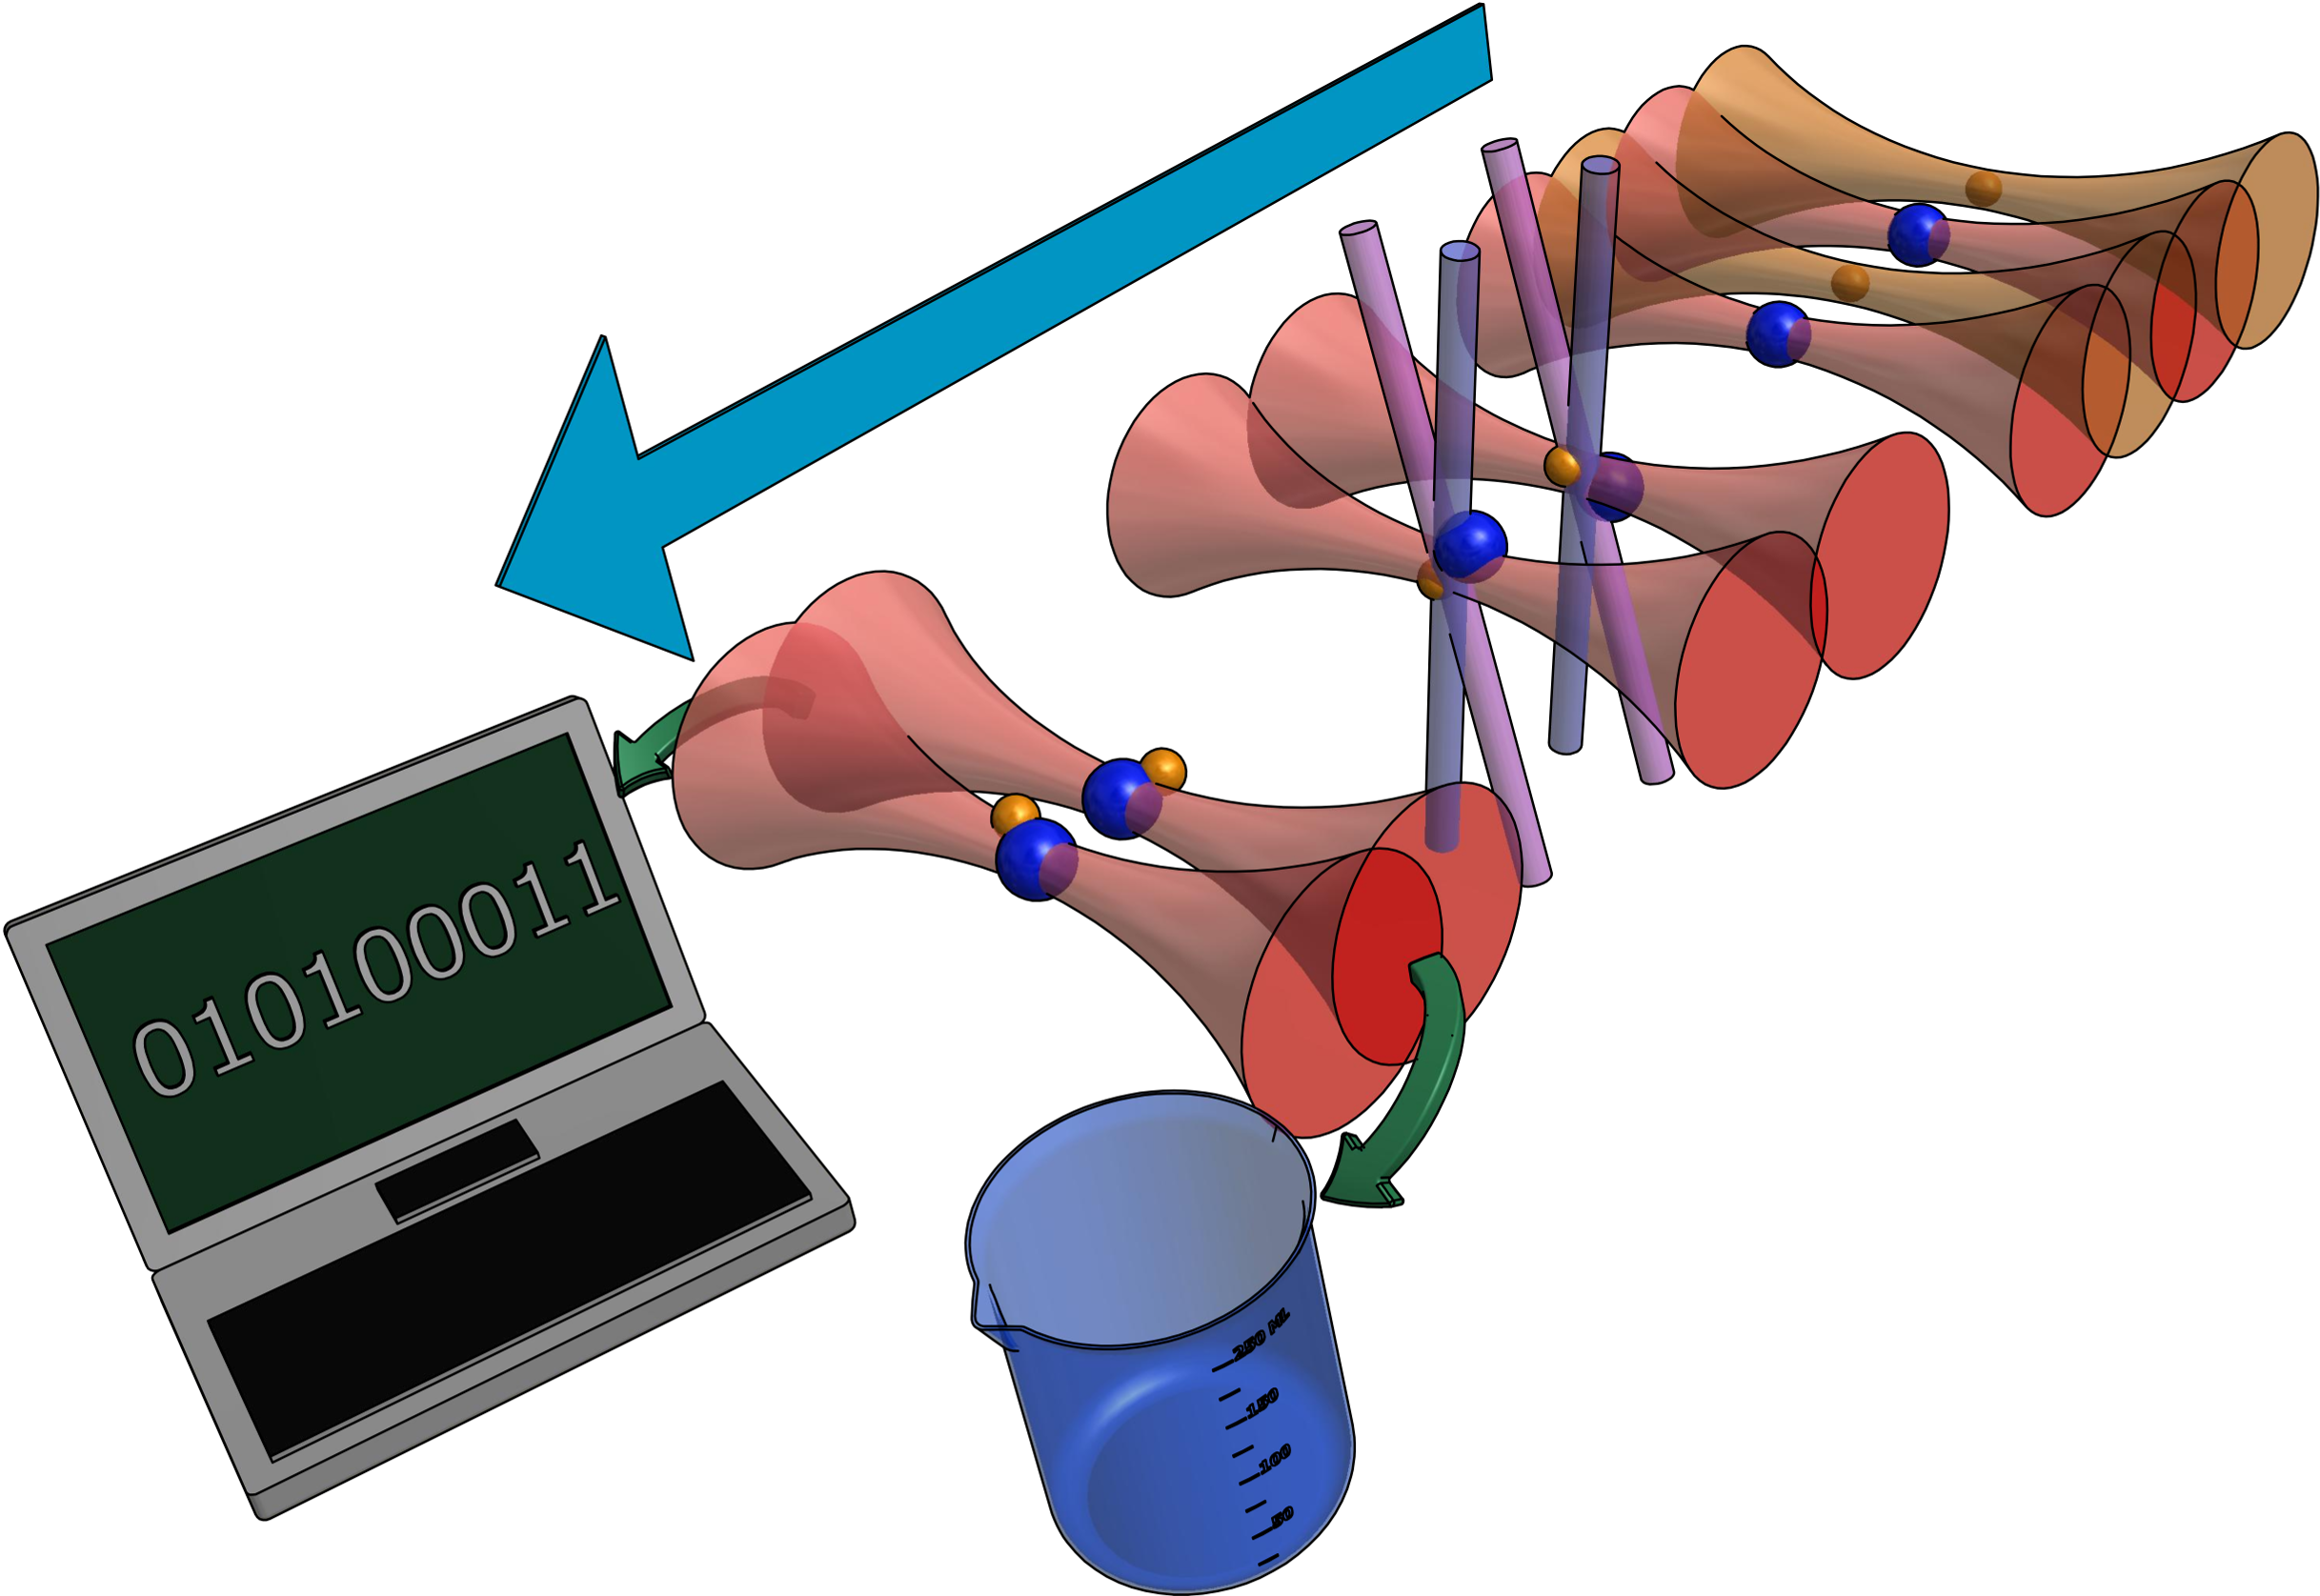
\includegraphics[width=8cm]{overall_full_min.png}
    \column{4cm}
    \begin{center}
      \usebeamercolor[fg]{title}{
        {\large{\theauthor}}\\
        {\small{\thedate}}\\
        {\small{\theinstitute}}}
    \end{center}
  \end{columns}
\end{frame}

% Done in Rb by ....
% - Load MOT
% - Trap with tweezer
% - Image
% Objective + EMCCD
% <figure 2> <animated>
% Didn't take so long for Cs (picture)
% <figure 3> Image, histogram

% 2.5min
\begin{frame}
  \begin{columns}[t]
    \column{5cm}
    \begin{block}{Procedure}
      \begin{itemize}
      \item<1-> MOT Loading
      \item<2-> Trapping
      \item<3-> Imaging
      \item<4-> Works for Cs
      \item<5-> Doesn't work for Na
      \end{itemize}
    \end{block}
    \column{7cm}
    \begin{center}
      \begin{tikzpicture}
        \visible<2-3>{
          \shade[shading=radial,rotate=90,yscale=1,fill opacity=0.6,
          inner color=red]
          plot[draw,samples=200,domain=-3:3] function {sqrt(0.0025 + x**2 / 10)}
          -- plot[draw,samples=200,domain=3:-3] function {-sqrt(0.0025 + x**2 / 10)};
          \path (0, 3) node[below] {Tweezer};
        }
        \visible<1-2>{
          \fill[orange,opacity=0.8,path fading=glow fading] (0,0) circle (1.5);
        }
        \visible<3>{
          \path (2, 0) node[align=center] {Imaging\\beams};
          \fill[orange,opacity=0.7,path fading=beam fading,transform canvas={rotate=25}]
          (-2, -0.2) rectangle (2, 0.2);
          \fill[orange,opacity=0.7,path fading=beam fading,transform canvas={rotate=-25}]
          (-2, -0.2) rectangle (2, 0.2);
        }
        \visible<2-3>{
          \fill [blue,path fading=glow fading] (0,0) circle (0.08);
        }
        \visible<4> {
          \path (0,0) node
          {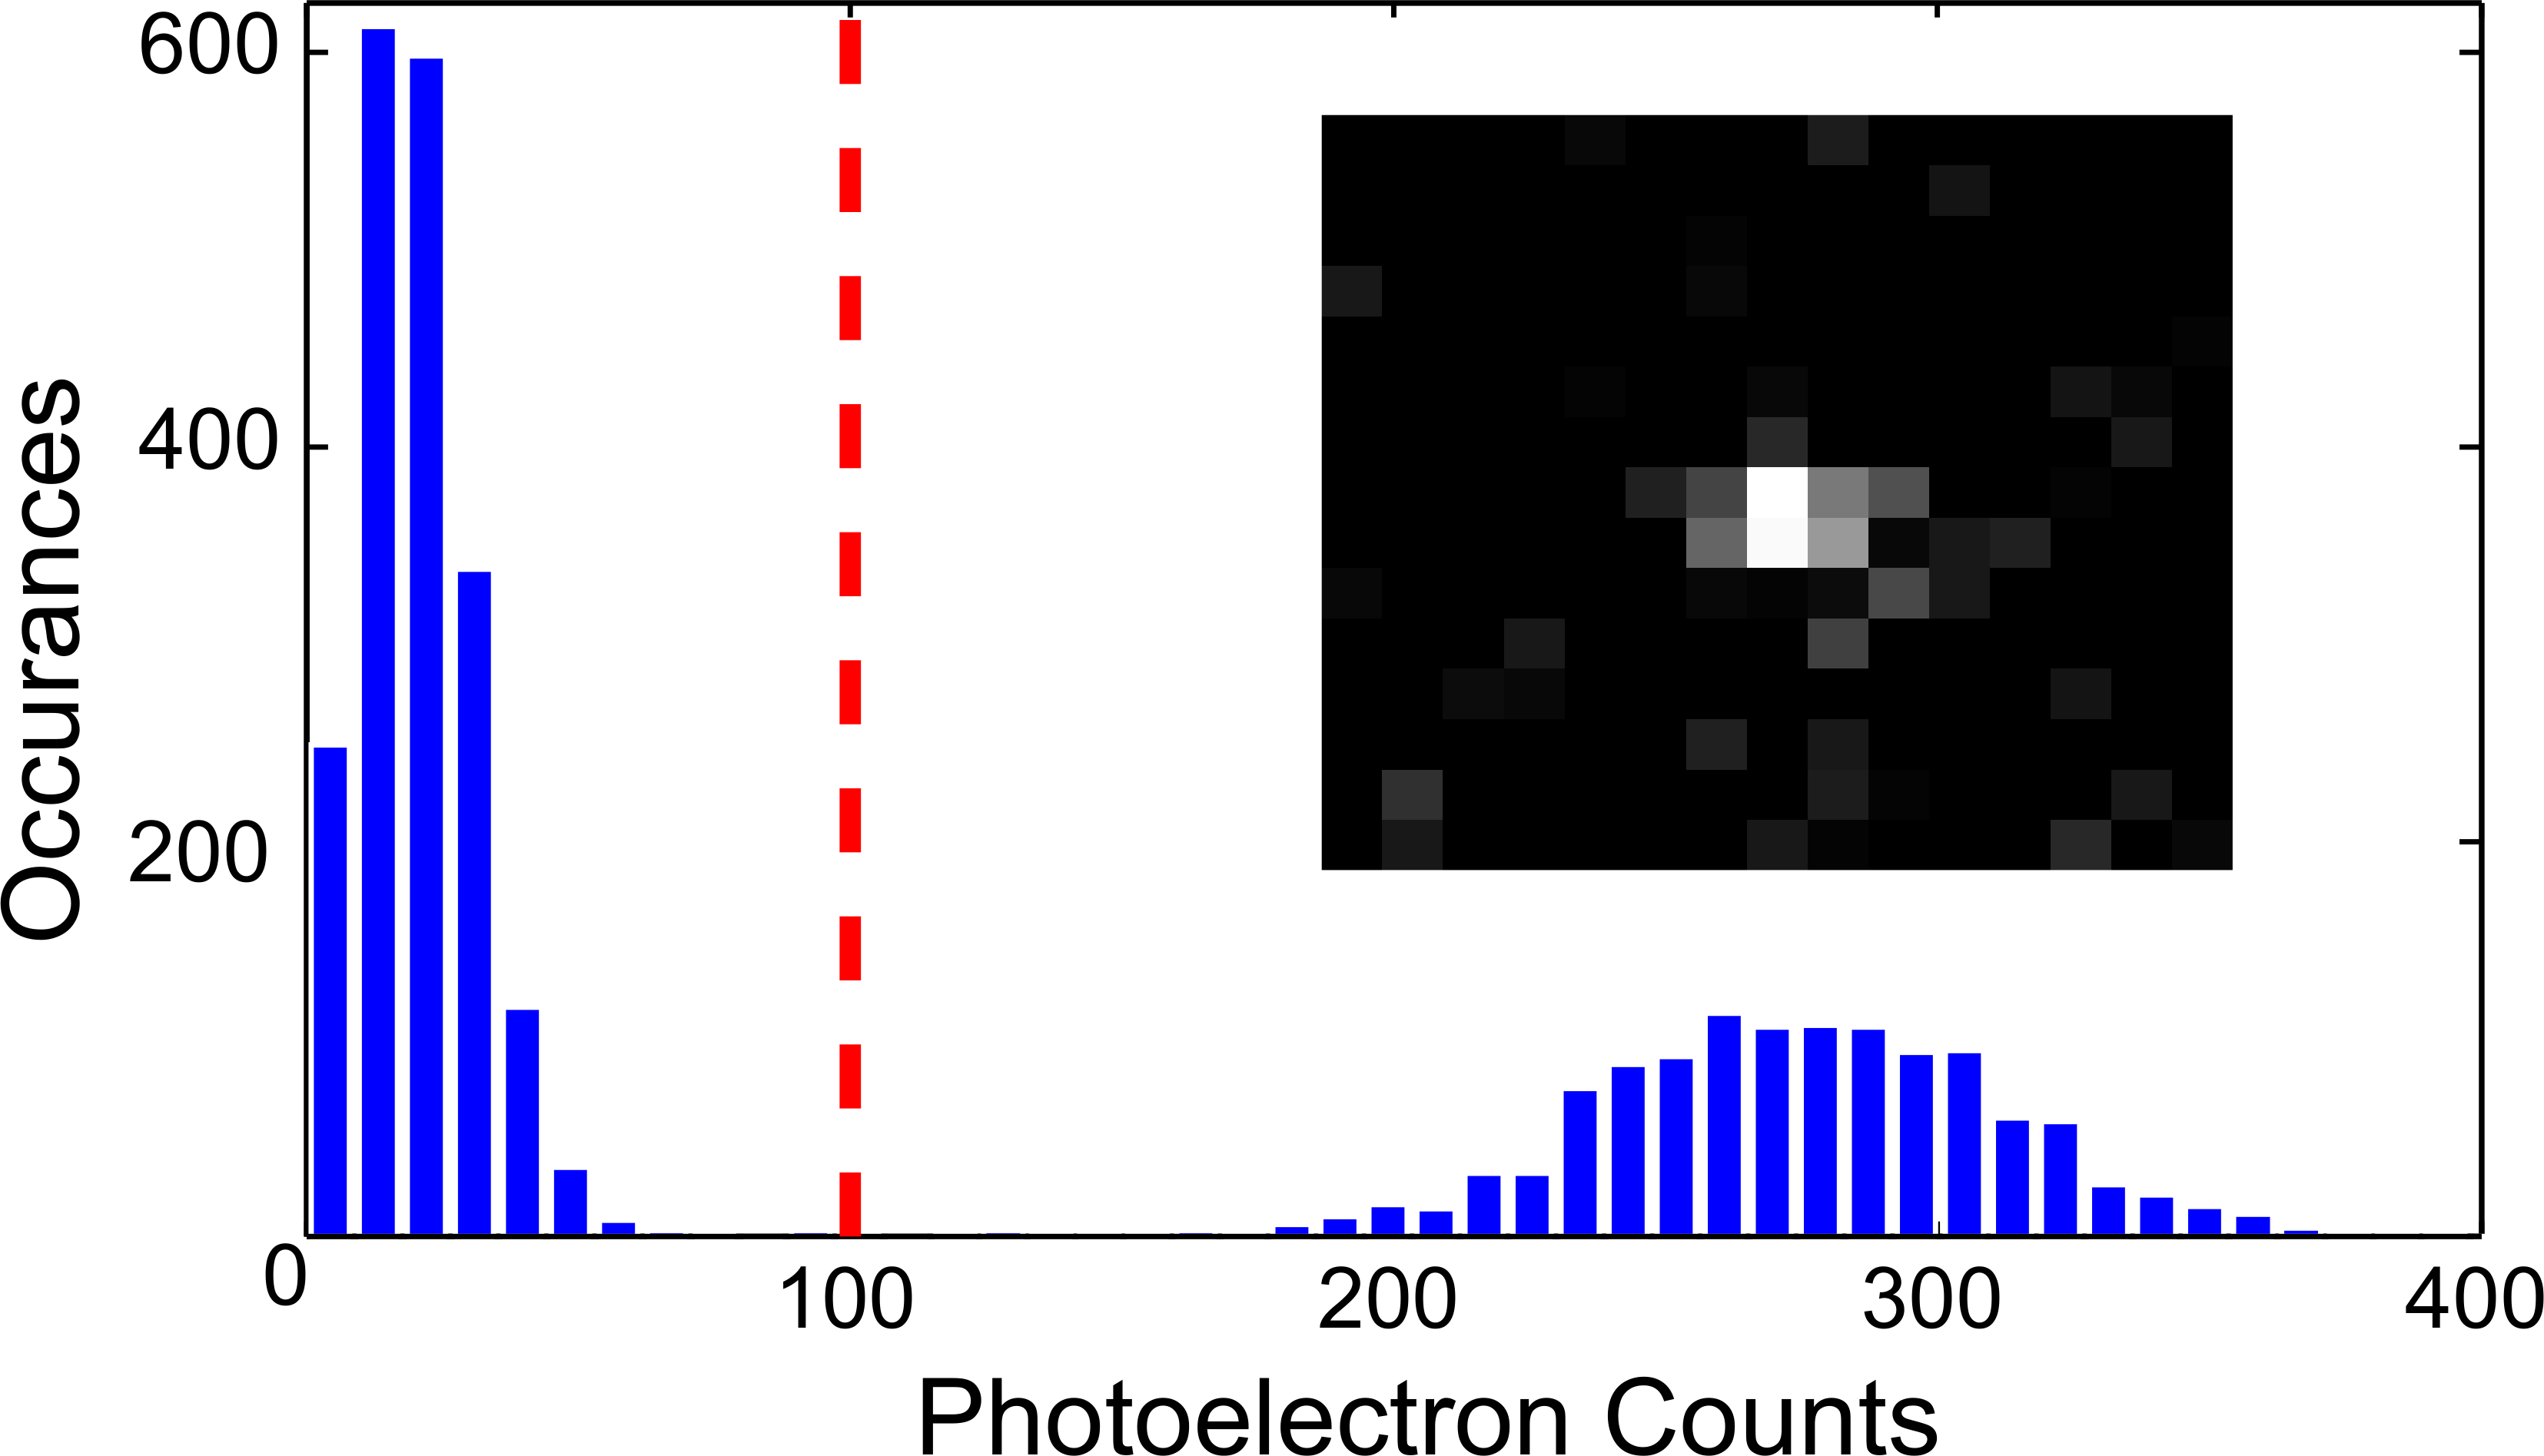
\includegraphics[width=7cm]{histogram.png}};
        }
      \end{tikzpicture}
    \end{center}
  \end{columns}
\end{frame}

% Doesn't work for Na
% We believe the issue is the difference between ground and excited state
% AC Stark shift.

% \beta parameter, due to multiple levels. 1 = magic

% Problems caused by this:
% 1. Loading
% -    Inefficient cooling
% -    Possibly reduced trap depth
% 2. Imaging
% -    + Off resonance

% 5min
\begin{frame}
  \begin{columns}
    \column{5cm}
    \begin{block}{Light shift}
      \begin{itemize}
      \item<2-> $\beta=\dfrac{\alpha_e}{\alpha_g}$ % Ratio between polarizability
      \item<4-> Inefficient cooling;\\
        Heating
      \item<5-> Shift imaging light out of resonance
      \end{itemize}
    \end{block}
    \visible<3-> {
      \begin{center}
        \begin{tabular}{|c|c|c|c|c|}
          \hline
          Atom&\multicolumn{3}{|c|}{Cs}&Na\\\hline
          $\lambda_{trap}$&922&935&970&700\\\hline
          $\beta_{cycle}$&2&1&0.6&-1\\\hline
        \end{tabular}
      \end{center}
    }
    \column{7cm}
    \begin{center}
      \begin{tikzpicture}
        \visible<-5> {
          % Excited state
          \draw[dashed,line width=1] (-2, 3) -- (2, 3);

          % \beta = 0.5
          \draw[violet,line width=1]
          plot[samples=200,domain=-2:2]
          function {3-0.5 * exp(-x**2 / 2 / (0.8**2))};

          \visible<2-> {
            \draw[dashed,line width=0.5] (2, 3) -- (2.5, 3) node[right] {$\beta=0$};

            % \beta = -1
            \draw[blue,line width=1]
            plot[samples=200,domain=-2:2]
            function {3+exp(-x**2 / 2 / (0.8**2))};

            \draw[blue,dashed,line width=0.5] (0, 4) -- (2.5, 4)
            node[right] {$\beta<0$};

            % \beta = 1
            \draw[black,line width=1]
            plot[samples=200,domain=-2:2]
            function {3-exp(-x**2 / 2 / (0.8**2))};
            \draw[black,dashed,line width=0.5] (0, 2) -- (2.5, 2)
            node[right] {$\beta=1$};

            % \beta = 1.67
            \draw[red,line width=1]
            plot[samples=200,domain=-2:2]
            function {3-1.67 * exp(-x**2 / 2 / (0.8**2))};
            \draw[red,dashed,line width=0.5] (0, 1.33) -- (2.5, 1.33)
            node[right] {$\beta>1$};
          }

          % Ground state
          \draw[dashed,line width=1] (-2, 0) -- (2, 0);
          \draw[black,line width=1]
          plot[samples=200,domain=-2:2]
          function {-exp(-x**2 / 2 / (0.8**2))};
        }
        \visible<6> {
          \path (0.5, 3) node[above] {
            \begin{tabular}{|c|c|c|c|}
              \multicolumn{4}{c}{Cs single atom loading}\\
              \hline
              $\lambda_{trap}$&922&935&970\\\hline
              Loading \%&$0$&$\approx50$&$\approx50$\\\hline
            \end{tabular}
          };
          \path (0.5, 2.5) node[below,align=center] {Cs single atom imaging\\
            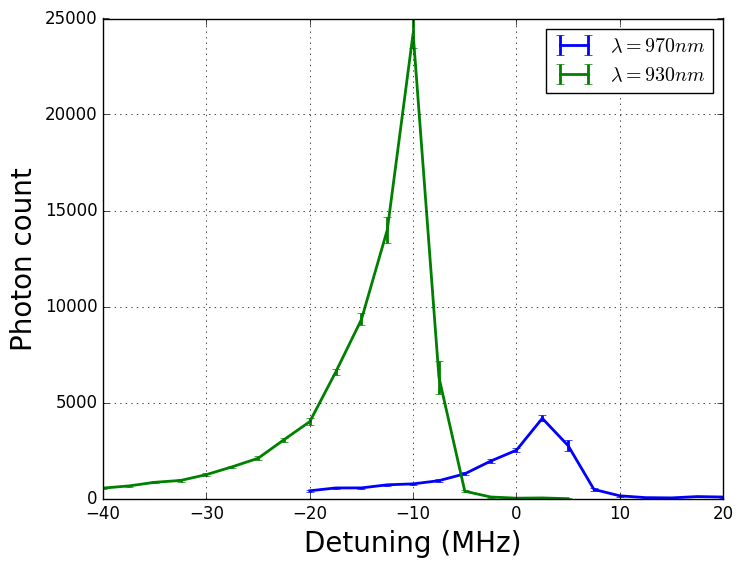
\includegraphics[width=6.5cm]{det-vs-photon-dc.png}};
        }
      \end{tikzpicture}
    \end{center}
  \end{columns}
\end{frame}

% Solution:
% * Switching
% * Fast enough (comparing to trap frequency)
% * Slow enough (comparing to excited stated lifetime)

\begin{frame}
  \begin{columns}
    \column{5cm}
    \begin{block}{Trap switching}
      \begin{itemize}
      \item<2-> Alternate between resonant and trap light
      \item<3-> Switching at $1-3$MHz\\
        {\small $f_{trap}=10\sim400$kHz}\\
        {\small $\Gamma=2\pi\times5\sim10$MHz}
      \item<7-> Being able to load single Na atom
      \end{itemize}
    \end{block}
      \begin{tikzpicture}
        \visible<2-7> {
          \path (0, 0) node {\includegraphics[width=6cm]{switching.png}};
        }
        \visible<8-> {
          \path (0, 0) node
          {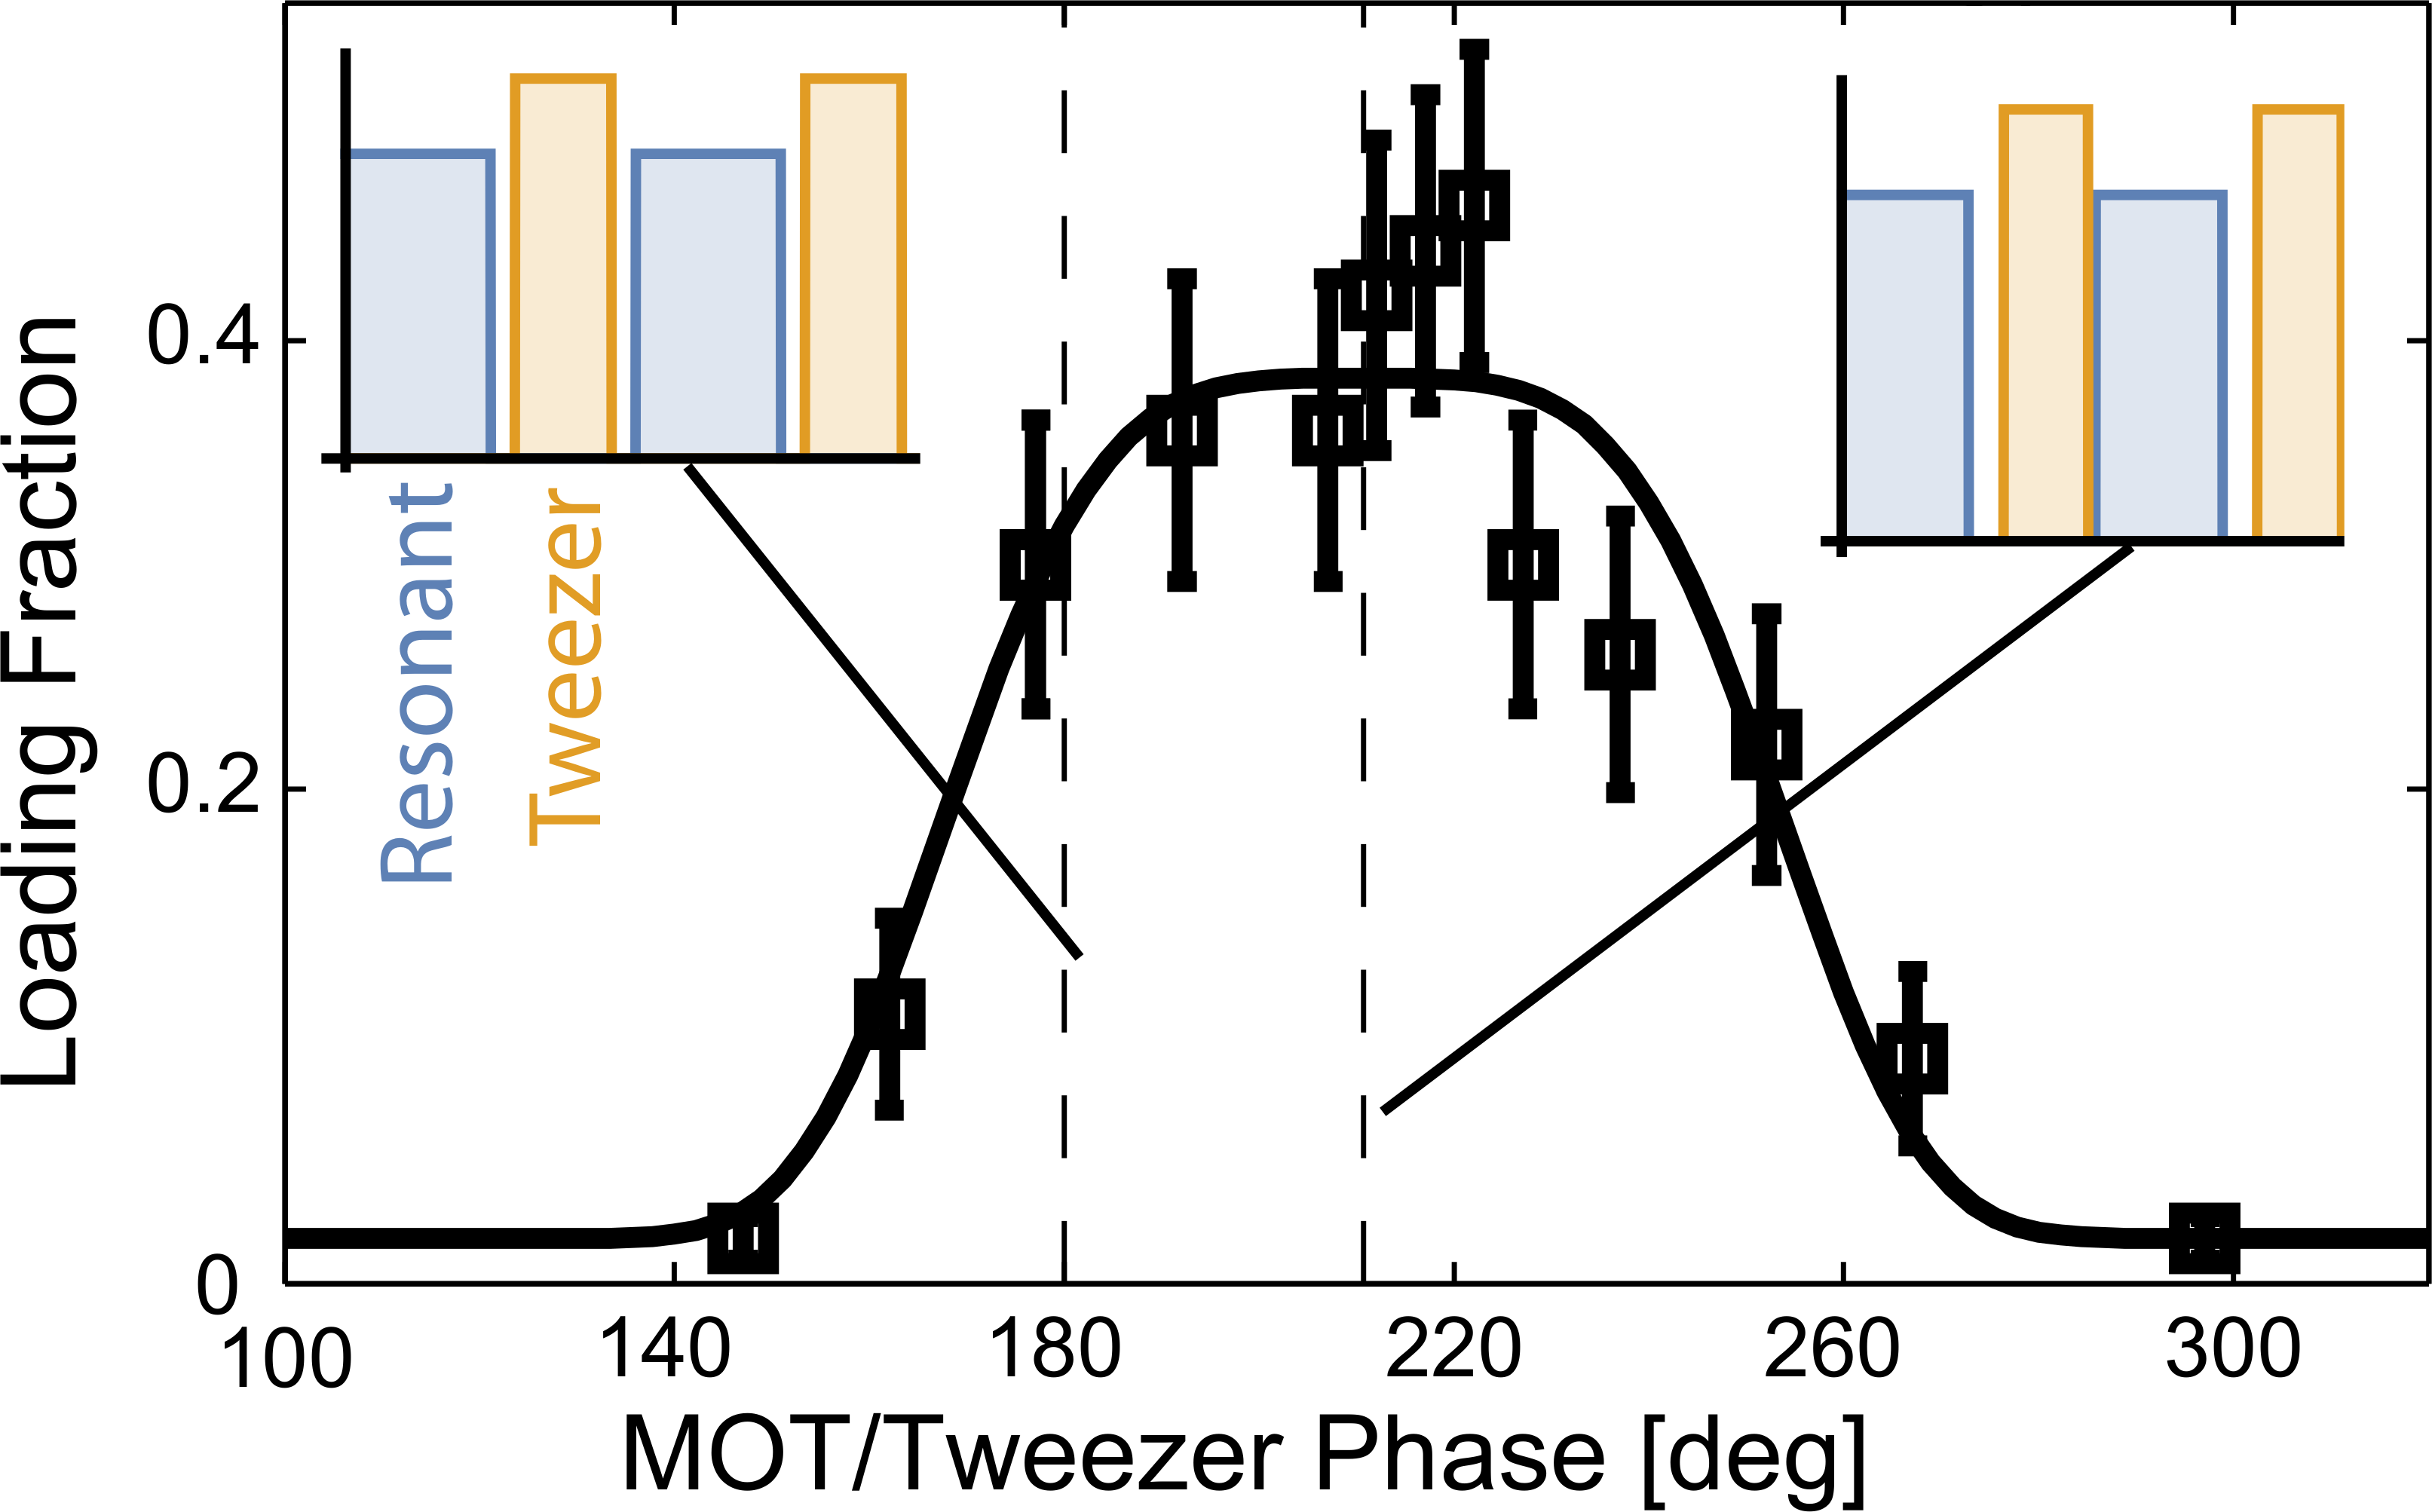
\includegraphics[width=5cm]{trap-phase.png}};
        }
      \end{tikzpicture}
    \column{7cm}
    \begin{center}
      \begin{tikzpicture}
        \visible<4-> {
          \path (0, 0) node[above,align=center]
          {
            \begin{tabular}{|c|c|c|c|}
              \multicolumn{4}{c}{Cs single atom loading}\\
              \hline
              $\lambda_{trap}$&922&935&970\\\hline
              Loading \%&{\color{red}$\approx50$}&$\approx50$&$\approx50$\\\hline
            \end{tabular}
          };
        }
        \visible<5> {
          \path (0, -0.5) node[below,align=center]
          {Cs single atom imaging\\
            \includegraphics[width=6cm]{det-vs-photon-dc2.png}};
        }
        \visible<6-> {
          \path (0, -0.5) node[below,align=center]
          {Cs single atom imaging\\
            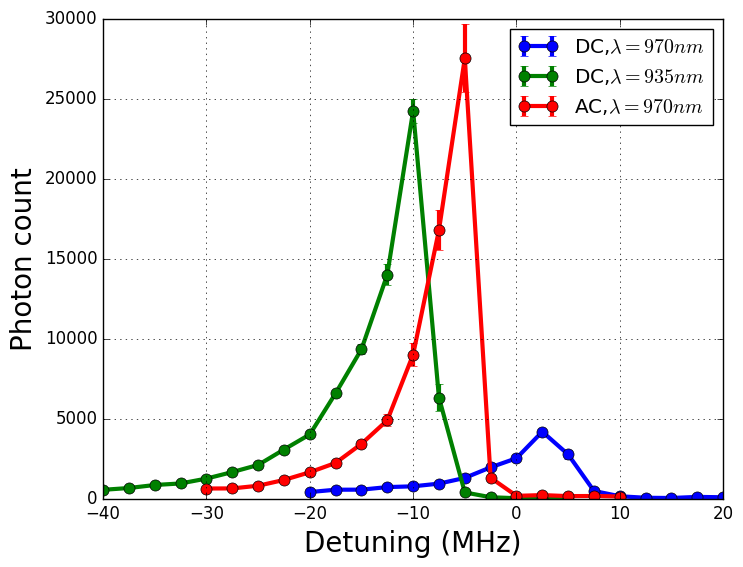
\includegraphics[width=6cm]{det-vs-photon-ac.png}};
        }
      \end{tikzpicture}
    \end{center}
  \end{columns}
\end{frame}

\begin{frame}[t]{Conclusion}
  \begin{itemize}
  \item Measured the effect of light shift on loading and imaging of single atom
  \item Overcome the light shift by alternating trapping and resonant light to achieve loading of single Na atom.
    % TODO: extension: Other species
  \end{itemize}
\end{frame}

\begin{frame}[t]
  % \vspace{-0.8cm}
  % \begin{columns}[t]
  %   \column{4cm}
  %   \begin{center}
  %     Prof. Kang-Kuen\\
  %     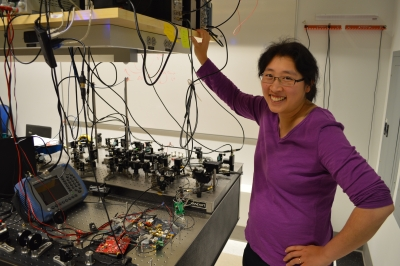
\includegraphics[width=3.5cm]{KangKuen.jpg}\\
  %     Nick (NaCs)\\
  %     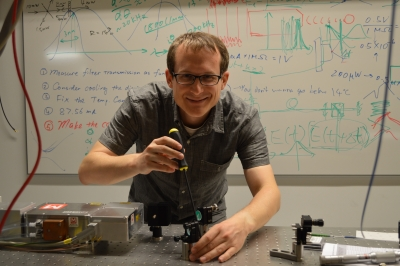
\includegraphics[width=3.5cm]{Nick.jpg}\\
  %     Lee (NaCs)\\
  %     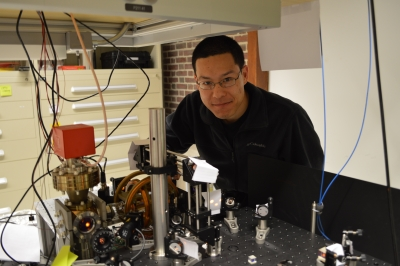
\includegraphics[width=3.5cm]{Lee.jpg}
  %   \end{center}
  %   \column{4cm}
  %   \begin{center}
  %     Yu (KRb)\\
  %     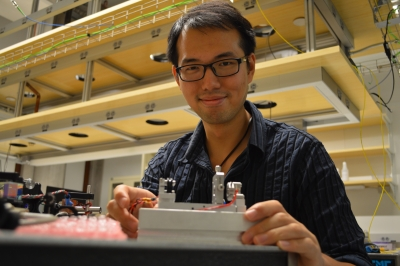
\includegraphics[width=3.5cm]{Yu.jpg}\\
  %     Hyungmok (KRb)\\
  %     \includegraphics[width=3.5cm]{Jim1.jpg}
  %   \end{center}
  %   \column{4cm}
  %   \begin{center}
  %     Saahil (Undergrad.)\\
  %     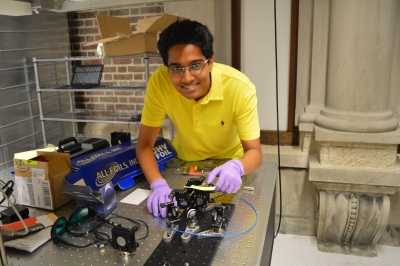
\includegraphics[width=3.5cm]{Saahil.jpg}\\
  %     Will (Undergrad.)\\
  %     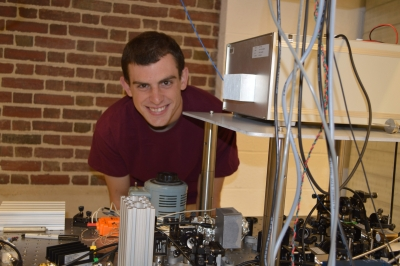
\includegraphics[width=3.5cm]{Will.jpg}
  %   \end{center}
  % \end{columns}
\end{frame}

\begin{frame}
\end{frame}

\end{document}
